\begin{center}
	\section{Resultados} \label{teorico:sed}
\end{center}


\subsection{Propiedades del fluido}

\noindent
\justify

Las Ecuaciones \ref{rhoH2O} y \ref{viscH2O} describen las propiedades termodin\'amicas del agua; y las Ecuaciones \ref{rhoEt} y \ref{viscEt} las del etanol a presi\'on atmosf\'erica en funci\'on de la temperatura del fluido $\left(\forall T \, \varepsilon [5 \degree C, 60 \degree C] \right)$. La Ecuaci\'on \ref{mezcla} permite predecir las propiedades de la mezcla agua - etanol a cualquier grado de concentraci\'on. Las propiedades de una mezcla agua - etanol al $50 \%$, $28 [\degree C]$, se pueden apreciar en el Cuadro \ref{temoM}.

\begin{table}[h!]
	\centering
	\begin{tabular}{|c|c|}
	\hline
	\textbf{Propiedad} & \textbf{Valor} \\ \hline
	$\rho _f \left[ kg / m^3 \right]$ & $889.4$ \\ \hline
	$\mu _f \left[ m^2 / s \right] $ & $1.06 * \, 10^{-6}$ \\ \hline
	\end{tabular}
	\caption{Propiedades de la mezcla agua - etanol al $50 \%$.}
	\label{temoM}
\end{table}

\subsection{Velocidad m\'axima de sedimentaci\'on}

\noindent
\justify

La velocidad m\'axima de sedimentaci\'on se calcula a trav\'es del procedimiento iterativo mostrado en la Figura \ref{UmaxS}. Los resultados de este procedimiento se pueden apreciar en la Figura \ref{iteraciones}.

\begin{table}[h!]
	\centering
	\begin{tabular}{|c|c|c|c|c|c|}
	\hline
	Iteraci\'on & $U_s [m/s]$ & $Re_s$ & $C$ & $U_c [m/s]$ & $Err_c [\%]$ \\ \hline
	1 & $1$ & $236.247$ & $0.637$ & $0.068$ & $93.159$ \\ \hline
	2 & $0.068$ & $16.162$ & $2.571$ & $0.034$ & $50.235$ \\ \hline
	3 & $0.034$ & $8.043$ & $4.382$ & $0.026$ & $23.397$ \\ \hline
	\multicolumn{6}{|c|}{$\cdots$} \\ \hline
	13 & $0.022$ & $5.115$ & $6.359$ & $0.022$ & $0.04 \, *10^{-1}$ \\ \hline	
	\end{tabular}
	\caption{Proceso de c\'alculo iterativo de la velocidad de sedimentaci\'on m\'axima.}
	\label{iteraciones}
\end{table}

\noindent
\justify

Se concluye que, con una estimaci\'on de error inferior al $0.01 \%$, la velocidad m\'axima de sedimentaci\'on es de $0.022 [m/s]$ con un n\'umero de Reynolds en la part\'icula de $5.115$.

\subsection{Geometr\'ia inicial}

\noindent
\justify

Con base en lo descrito en las secciones \ref{geoLa}, \ref{anchoSed}, \ref{Rev0} y \ref{enTol} la geometr\'ia del sistema de sedimentaci\'on de placas inclinadas presenta las siguientes dimensiones:

\begin{table}[h!]
	\centering
	\begin{tabular}{|c|c|}
		\hline
		\textbf{Par\'ametro} & \textbf{Valor} \\ \hline
			Ancho lamela $[cm]$ & $5$ \\ \hline
			Longitud lamela $[cm]$ & $40$ \\ \hline
			Separaci\'on entre lamelas $[cm]$ & $2.5$ \\ \hline
			Inclinaci\'on $[\degree]$ & $60$ \\ \hline
			N\'umero lamelas & $5$ \\ \hline
			Ancho panel $[cm]$ & $2.2$ \\ \hline
			Di\'ametro de entrada $[cm]$ & $27$ \\ \hline
			Altura total $[cm]$ & $105$ \\ \hline
	\end{tabular}
	\caption{Geometr\'ia de estudio}
	\label{GeoInicial}
\end{table}

\noindent
\justify

Es posible apreciar la geometr\'ia de an\'alisis en la Figura \ref{geometry}; destacando: una zona de \textit{entrada} de la mezcla s\'olido - l\'iquido; una de \textit{salida} (al final de la superficie inclinada), en donde se espera obtener la \textit{fase l\'iquida} de la mezcla y un \'area de dep\'osito de lodos, localizada en la parte inferior de la geometr\'ia. El \textbf{\'area sombreada} corresponde a la regi\'on de inter\'es en donde se desarrollan las simulaciones num\'ericas.

%Datos geométricos
\def\D{2.7}    	%Diámetro de ingreso
\def\H{3}		%Altura de la zona de lodos
\def\A{2.5}		%Ancho del panel de lamelas
\def\HL{3}		%Altura del panel de lamelas
\def\nL{5}		%Número de lamelas
\def\ang{60}	%Ángulo de inclinación del panel

\def\xlam{\x+\A+0.5*\D}

\def\fin{\nL-1}

%Inclinación
%\def\xL{{\HL*cos(\ang)}}

%Referencia
\def\x{-\A/2-0.5/2*\D-\HL/2}
\def\y{0}

\begin{figure}[h!]
	\centering
	\begin{adjustbox}{max width = \textwidth}
	\begin{tikzpicture}
		%Geometría general
		\draw (\x,\y) -- (\x,-\D) -- (\x+0.5*\D,-\D) --
			(\x+0.5*\D, -2*\D) -- ({\x+0.5*\D + \A/3}, -2.5*\D) -- ({\x+0.5*\D + 2*\A/3}, -2.5*\D) -- (\x+\A+0.5*\D, -2*\D) -- 
			(\x+\A+0.5*\D, \y) -- ({\xlam + \HL*cos(\ang)},{\y + \HL*sin(\ang)}) -- ({\xlam + \HL*cos(\ang) - \A}, {\y + \HL*sin(\ang)}) -- (\xlam - \A, \y) -- cycle;
						
		%Lamelas
		\foreach \xL in {1, ..., \nL}
			\draw (\xlam - \xL*\A/\nL,\y) -- ({\xlam + \HL*cos(\ang) - \xL*\A/\nL}, {\y + \HL*sin(\ang)});
		\foreach \xL in {1, ..., \nL}	
			\draw[dashed, step=0.5cm, blue!60!green, pattern=north west lines, pattern color=blue!60!green] ({\xlam - (\xL-1)*\A/\nL},\y) -- (\xlam - \xL*\A/\nL,\y) -- ({\xlam + \HL*cos(\ang) - \xL*\A/\nL}, {\y + \HL*sin(\ang)}) -- ({\xlam + \HL*cos(\ang) - (\xL-1)*\A/\nL}, {\y + \HL*sin(\ang)})  -- cycle;
			
		%Dimensiones
		\draw (\x+0.5*\D + 0.1, -2*\D) -- (\x, -2*\D);
		\draw[arrows={-Triangle[angle=90:3pt,red!10!black,fill=red!10!black]}] (\x+0.25*\D, -2*\D) -- (\x+0.25*\D, -\D);
		\draw[arrows={-Triangle[angle=90:3pt,red!10!black,fill=red!10!black]}] (\x+0.25*\D, -\D)  -- (\x+0.25*\D, -2*\D);
		\node[align=left] at (\x-0.1, -3/2*\D) {$29.4 [cm]$};
		
		\draw (\x+0.5*\D + 0.1 + \A, -2*\D) -- (\x+\D + 0.1 + \A, -2*\D);
		\draw (\x+0.5*\D + 0.1 + \A, \y) -- (\x+1.5*\D + 0.1 + \A, \y);
		
		\draw[arrows={-Triangle[angle=90:3pt,red!10!black,fill=red!10!black]}] (\x+0.75*\D + \A, -2*\D) -- (\x+0.75*\D+ \A, \y);
		\draw[arrows={-Triangle[angle=90:3pt,red!10!black,fill=red!10!black]}] (\x+0.75*\D+ \A, \y) --  (\x+0.75*\D+ \A, -2*\D);
		
		\node[align=right] at (\x+1.05*\D+ \A, -\D) {$56.4 [cm]$};
		
		\draw ({\xlam + \HL*cos(\ang)},{\y + \HL*sin(\ang)}) -- ({\xlam + \HL*cos(\ang) + \D},{\y + \HL*sin(\ang)});

		\draw (\x+0.5*\D, -2*\D - 0.1) -- (\x+0.5*\D, -2.8*\D - 0.1);
		\draw (\x+0.5*\D + \A, -2*\D - 0.1) -- (\x+0.5*\D + \A, -2.8*\D - 0.1);	
		\draw[arrows={-Triangle[angle=90:3pt,red!10!black,fill=red!10!black]}] (\x+0.5*\D + \A, -2.6*\D-0.1) -- (\x+0.5*\D, -2.6*\D - 0.1);
		\draw[arrows={-Triangle[angle=90:3pt,red!10!black,fill=red!10!black]}] (\x+0.5*\D, -2.6*\D - 0.1) -- (\x+0.5*\D + \A, -2.6*\D-0.1);
		
		\node at (\x+0.5*\D + \A/2, -2.7*\D - 0.1) {$35 [cm]$};	
		
		\draw[arrows={-Triangle[angle=90:3pt,red!10!black,fill=red!10!black]}] ({\xlam + \HL*cos(\ang) + \D/4}, {\y + \HL*sin(\ang)}) -- ({\xlam + \HL*cos(\ang) + \D/4}, \y);
		
		\draw[arrows={-Triangle[angle=90:3pt,red!10!black,fill=red!10!black]}] ({\xlam + \HL*cos(\ang) + \D/4}, \y) --  ({\xlam + \HL*cos(\ang) + \D/4}, {\y + \HL*sin(\ang)});
		
		\node at ({\xlam + \HL*cos(\ang) + \D/4 + 0.75}, {\y + \HL*sin(\ang)/2}) {$34.6 [cm]$};
		
		%Área de interés
		\draw[dashed, step=0.5cm, blue!60!green, pattern=north west lines, pattern color=blue!60!green] (\x,\y) -- (\x,-\D) -- (\x+0.5*\D,-\D) -- (\x+0.5*\D, -2*\D) -- (\x+\A+0.5*\D, -2*\D) -- (\x+\A+0.5*\D, \y) -- cycle;
		
		%Señalización
		\draw[red!10!black, arrows={-Triangle[angle=90:3pt,red!10!black,fill=red!10!black]}] (\x-2,-\D/2) node[above] {Entrada \textit{mezcla}} -- (\x-0.5,-\D/2);
		
		\draw[red!10!black, arrows={-Triangle[angle=90:3pt,red!10!black,fill=red!10!black]}] ({\xlam + \HL*cos(\ang) - \A/\nL/2},{\y + \HL*sin(\ang)}) node[above] {Salida \textit{fase l\'iquida}} -- ({\xlam + (\HL+1)*cos(\ang) - \A/\nL/2},{\y + (\HL+1)*sin(\ang)});
		
		
	\end{tikzpicture}
	\end{adjustbox}
	\caption{Vista en corte de la geometr\'ia del sistema de sedimentaci\'on.}
	\label{geometry}
\end{figure}

\noindent
\justify

Con base en la geometr\'ia descrita en el Cuadro \ref{GeoInicial}, se obtuvieron los siguientes par\'ametros operacionales:

\begin{itemize}
	\item $v_0 = 1.014 [cm/s]$
	\item $Re = 478.993$
	\item $U_c = 0.208 [cm/s]$
\end{itemize}

\subsection{Mallado}

\noindent
\justify

Gran parte del \'exito de las simulaciones num\'ericas recaen en la discretizaci\'on del dominio y en la calidad de los elementos que la componen$^{\cite{Roda-Casanova2021}}$. Se desarroll\'o una metodolog\'ia de mallado autom\'atico con base en el lenguaje \textit{gmsh} tomando como variables de entrada las dimensiones de la geometr\'ia definida en la secci\'on \ref{geo}. Esta metodolog\'ia emplea elementos de diferentes tama\~nos y permite tambi\'en definir su naturaleza (rectangulares o triangulares).

\noindent
\justify

El algoritmo ejecuta, adem\'as, un refinamiento autom\'atico en la zona en donde ocurre el mayor grado de sedimentaci\'on: en la superficie inclinada, como se aprecia en la Figura \ref{malla:geo}.

\begin{figure}[h!]
	\centering
	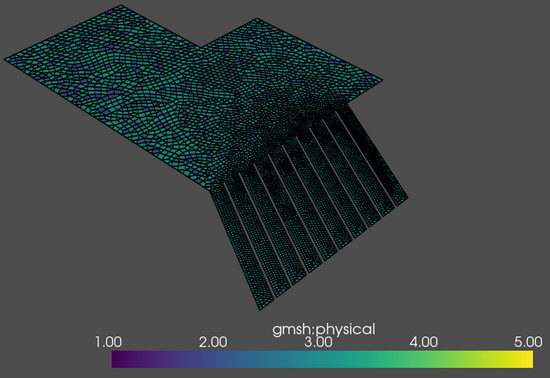
\includegraphics[width=\textwidth]{Images/CFDEM/malla2.png}
	\caption{Mallado de la geometr\'ia.}
	\label{malla:geo}
\end{figure}

\newpage

\noindent
\justify

La malla mostrada en la Figura \ref{malla:geo} presenta las siguientes caracter\'isticas:

\begin{table}[h!]
	\centering
	\begin{tabular}{|c|c|}
		\hline
		\textbf{Par\'ametro} & \textbf{Valor} \\ \hline
		Tipo de elementos & Rectangulares \\ \hline
		N\'umero de elementos & 20415 \\ \hline
		N\'umero de nodos & 13692 \\ \hline	
	\end{tabular}
	\caption{Datos de la malla generada.}
	\label{malla}
\end{table}

\noindent
\justify

Al emplear el m\'etodo \texttt{checkMesh} de OpenFOAM para el an\'alisis preliminar de malla, se obtuvieron los siguientes resultados:

\begin{table}[h!]
	\centering
	\begin{tabular}{|c|c|}
		\hline
		\textbf{Par\'ametro} & \textbf{Valor} \\ \hline
		Apertura \textit{m\'axima} entre elementos & 11.45 \\ \hline
		Checkeo de \textit{no} ortogonalidad & OK \\ \hline
		Oblicuidad m\'axima & 0.66 OK \\ \hline
		Conclusi\'on de malla & OK \\ \hline
	\end{tabular}
	\caption{Resumen de resultados sobre el checkeo de malla.}
	\label{check}
\end{table}

\noindent
\justify

A partir de los resultados mostrados en el Cuadro \ref{check}, se concluye que la malla es \'optima para el desarrollo de las simulaciones num\'ericas consecutivas.

\subsection{Condiciones de frontera}

\noindent
\justify

Complementando la informaci\'on descrita en la secci\'on \ref{CondF}, las condiciones de frontera del problema se resumen en el Cuadro \ref{condFr}.

\begin{table}[h!]
	\centering
	\begin{tabular}{|c|c|c|c|}
		\hline
		\textbf{Zona} & \textbf{Propiedad} & \textbf{Valor}  & \textbf{Tipo} \\ \hline
		\textit{Entrada} & Velocidad $[m/h]$ & $3.493$ & Neumann \\ \hline
		\textit{Salida} & Presi\'on $[KPa]$ & $101.325$ & Dirichlet \\ \hline
	\end{tabular}
	\caption{Clasificaci\'on de las condiciones de frontera.}
	\label{condFr}
\end{table}

\newpage

\subsection{Simulaci\'on CFD}

\noindent
\justify

Con base en la metodolog\'ia descrita en la secci\'on \ref{MetCFD}, se emple\'o el solucionador \texttt{pimpleFOAM} de OpenFOAM; obteniendo los siguientes resultados:

\begin{figure}[h!]
	\centering
	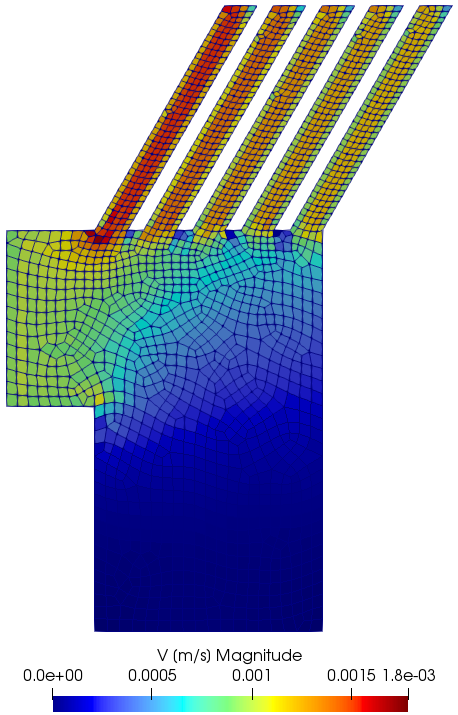
\includegraphics[width=0.33\textwidth]{Images/CFD/vel1.png}
	\caption{Diagrama de contorno de la distribuci\'on de velocidades del sistema de sedimentaci\'on.}
	\label{CFD:vel}
\end{figure}

\begin{figure}[h!]
	\centering
	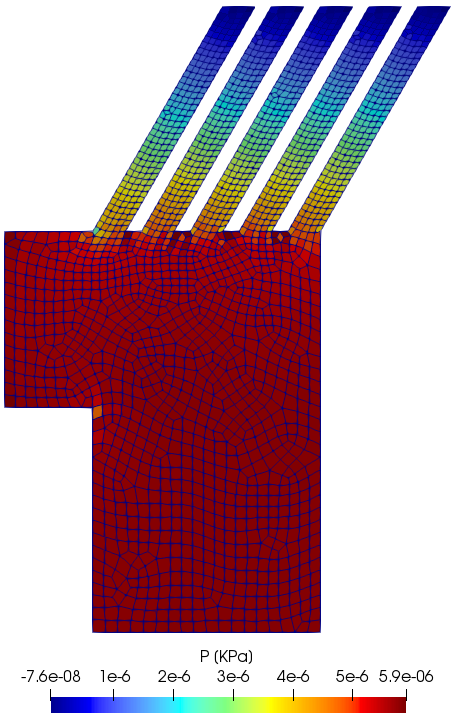
\includegraphics[width=0.33\textwidth]{Images/CFD/p1.png}
	\caption{Diagrama de contorno de la distribuci\'on de presiones del sistema de sedimentaci\'on.}
	\label{CFD:p}
\end{figure}

\subsection{Error computacional}

\noindent
\justify

De acuerdo a lo estipulado en la secci\'on \ref{SimuErr}, se desarroll\'o un refinamiento de malla para calcular el error de la simulaci\'on num\'erica. El resumen de resultados se puede apreciar en el Cuadro \ref{resumErr}.

\begin{table}[h!]
	\centering
	\begin{tabular}{|c|c|c|c|c|}
		\hline
		\textbf{Iteraci\'on} & \textbf{N\'um. nodos} & \textbf{Vel. m\'ax.$[m/s]$} & \textbf{P. m\'ax. $[KPa]$} & \textbf{Error m\'ax.} \\ \hline
		1 & $4560$ & $17.82 \cdot 10 ^{-3}$ & $5.90 \cdot 10 ^{-6}$ & $12.98 \%$ \\ \hline
		2 & $8832$ & $19.66 \cdot 10 ^{-3}$ & $6.78 \cdot 10 ^{-6}$ & $5.83 \%$ \\ \hline
		3 & $17636$ & $20.50 \cdot 10 ^{-3}$ & $ 7.20 \cdot 10 ^{-6}$ & $3.17 \%$ \\ \hline
		4 & $36820$ & $19.87 \cdot 10 ^{-3}$ & $7.25 \cdot 10 ^{-6}$ & - \\ \hline
	\end{tabular}
	\caption{Resultados del proceso iterativo.}
	\label{resumErr}
\end{table}

\noindent
\justify

En la Figura \ref{resumErrG}, se puede apreciar la tendencia del error de velocidad m\'axima de forma gr\'afica.

\begin{figure}[h!]
	\centering
	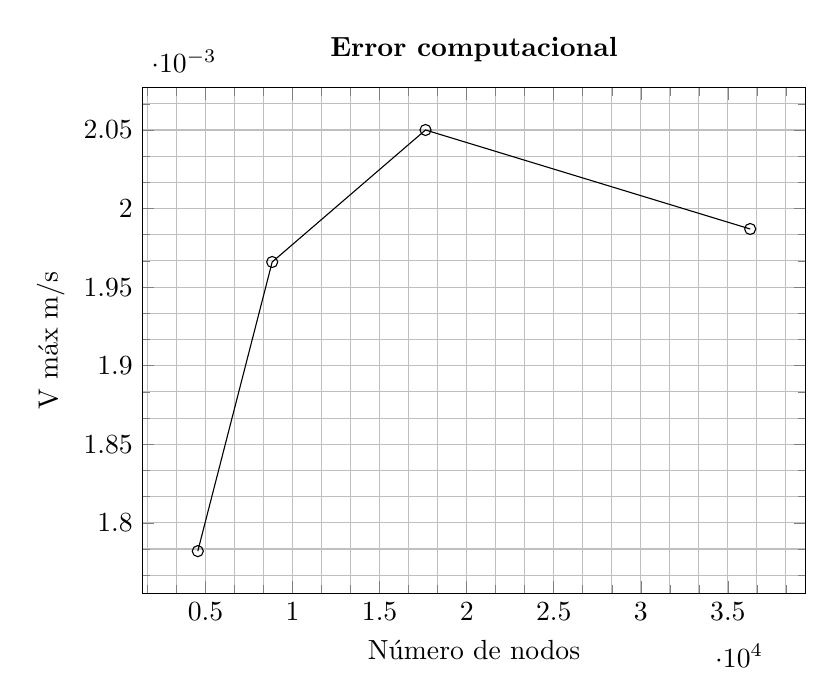
\begin{tikzpicture}
		\begin{axis}[
			grid = both, minor tick num=2,
			title = \textbf{Error computacional},
			xlabel = N\'umero de nodos,
			ylabel = V m\'ax m/s,
			legend pos = outer north east,
			width=10cm, height=8cm
		]
		%\addplot[blue, line width=2pt] {\val};
		\addplot[
        scatter,scatter src=explicit symbolic,
        scatter/classes={
            a={mark=o,black},
            b={mark=triangle*,red},
            c={mark=o,draw=black,fill=black}
        }
    ]
    table[x=x,y=y,meta=label]{
        x	y	label
		4560	0.001782	a
		8832	0.001966	a
		17636	0.002050	a
		36280	0.001987	a
    };
		%\legend{Te\'orico, Num\'erico};
		\end{axis}
	\end{tikzpicture}
	\caption{Cambio de la velocidad m\'axima con respecto al refinamiento de malla.}
	\label{resumErrG}
	\end{figure}

\noindent
\justify

En la Figura \ref{resumErrGP}, se puede apreciar la tendencia del error en la presi\'on m\'axima de forma gr\'afica.

\begin{figure}[h!]
	\centering
	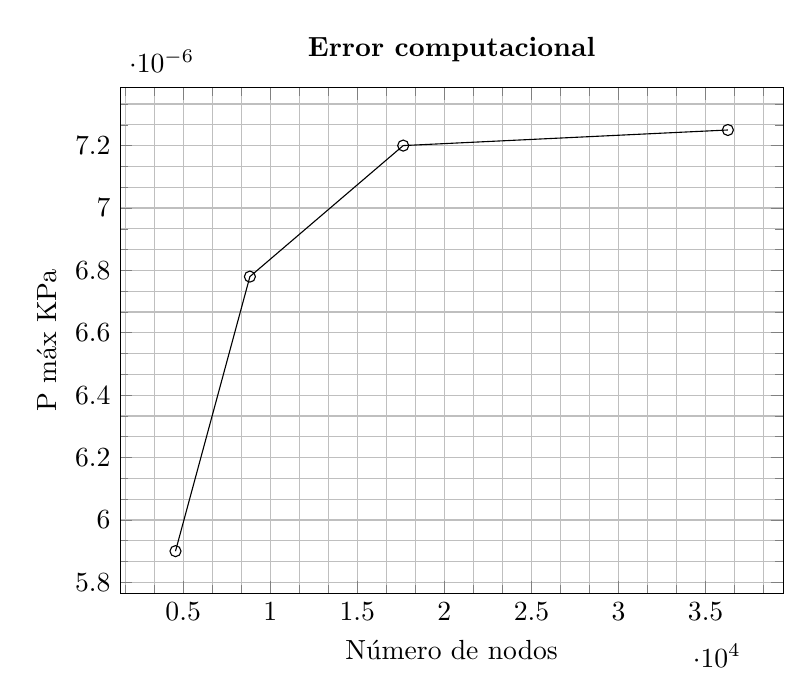
\begin{tikzpicture}
		\begin{axis}[
			grid = both, minor tick num=2,
			title = \textbf{Error computacional},
			xlabel = N\'umero de nodos,
			ylabel = P m\'ax KPa,
			legend pos = outer north east,
			width=10cm, height=8cm
		]
		%\addplot[blue, line width=2pt] {\val};
		\addplot[
        scatter,scatter src=explicit symbolic,
        scatter/classes={
            a={mark=o,black},
            b={mark=triangle*,red},
            c={mark=o,draw=black,fill=black}
        }
    ]
    table[x=x,y=y,meta=label]{
        x	y	label
		4560	5.90e-6		a
		8832	6.78e-6		a
		17636	7.20e-6		a
		36280	7.25e-6 	a
    };
		%\legend{Te\'orico, Num\'erico};
		\end{axis}
	\end{tikzpicture}
	\caption{M\'etodo de validaci\'on simple.}
	\label{resumErrGP}
	\end{figure}

\noindent
\justify

Cabe destacar, con base en las Figuras \ref{CFD:vel} y \ref{CFD:p}, que la presi\'on m\'axima se encuentra entre la zona de entrada de la mezcla y la zona de dep\'osito de los sedimentos; mientras que la velocidad m\'axima se encuentra en la primera lamela de izquierda a derecha. Con base en los resultados reportados en el Cuadro \ref{resumErr}, y las Figuras \ref{resumErr} y \ref{resumErrG}, se escoge la malla de $17636$ nodos para el desarrollo de la simulaci\'on CFD-DEM.

\subsection{Simulaci\'on CFD-DEM}

\noindent
\justify

La informaci\'on referente a la malla empleada para el desarrollo de la simulaci\'on CFD-DEM se puede apreciar en el Cuadro \ref{mallaF}.

\begin{table}[h!]
	\centering
	\begin{tabular}{|c|c|}
		\hline
		\textbf{Par\'ametro} & \textbf{Valor} \\ \hline
		Tipo de elementos & Rectangulares \\ \hline
		N\'umero de elementos & 23587 \\ \hline
		N\'umero de nodos & 17636 \\ \hline
		Tama\~no m\'aximo de elementos $[\mu m]$ & $10000$ \\ \hline
		Tama\~no m\'inimo $[\mu m]$ & $5000$ \\ \hline	
	\end{tabular}
	\caption{Datos de la malla inicial generada.}
	\label{mallaF}
\end{table}

\noindent
\justify

Se emple\'o un refinamiento de malla en las lamelas que corresponden a $5000 [\mu m]$ de tama\~no m\'inimo. 

\noindent
\justify

La validaci\'on de malla a trav\'es del comando \texttt{checkMesh} de OpenFOAM presenta los siguientes resultados:

\begin{table}[h!]
	\centering
	\begin{tabular}{|c|c|}
		\hline
		\textbf{Par\'ametro} & \textbf{Valor} \\ \hline
		Apertura \textit{m\'axima} entre elementos & 11.65 \\ \hline
		Checkeo de \textit{no} ortogonalidad & OK \\ \hline
		Oblicuidad m\'axima & 0.79 OK \\ \hline
		Conclusi\'on de malla & OK \\ \hline
	\end{tabular}
	\caption{Resumen de resultados sobre el checkeo de malla.}
	\label{check}
\end{table}

\noindent
\justify

En la Figura \ref{CFDEM:fpart} se puede apreciar el comportamiento fluido - part\'icula del sistema de sedimentaci\'on en $t = 60 [s]$.

\begin{figure}[h!]
	\centering
	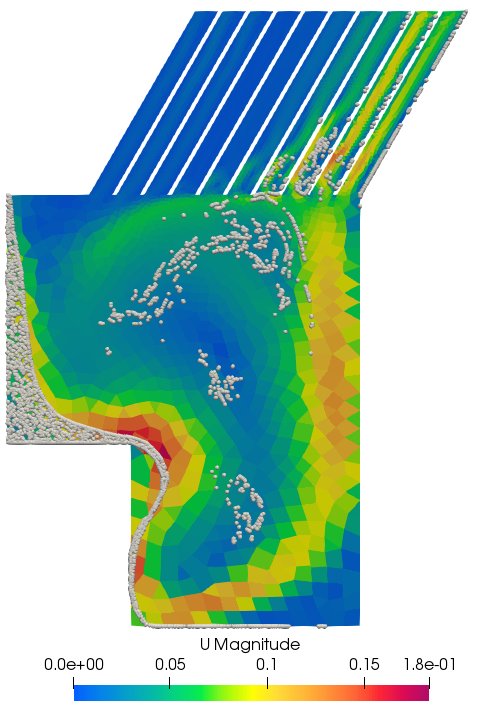
\includegraphics[width=0.5\textwidth]{Images/CFDEM/simu1.png}
	\caption{Simulaci\'on CFD-DEM $\rightarrow$ interacci\'on fluido-part\'icula.}
	\label{CFDEM:fpart}
\end{figure}

\noindent
\justify

Los resultados de los diagramas de contorno de velocidad y de presi\'on, en $t = 60 [s]$, se pueden apreciar en las Figuras \ref{CFDEM:vel} y \ref{CFDEM:p}.

\begin{figure}[h!]
	\centering
	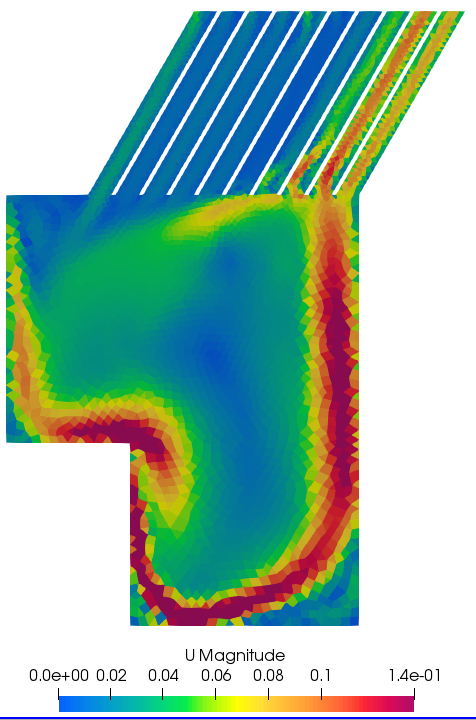
\includegraphics[width=0.42\textwidth]{Images/CFDEM/vel.png}
	\caption{Diagrama de contorno de velocidad $t = 60 [s]$.}
	\label{CFDEM:vel}
\end{figure}

\begin{figure}[h!]
	\centering
	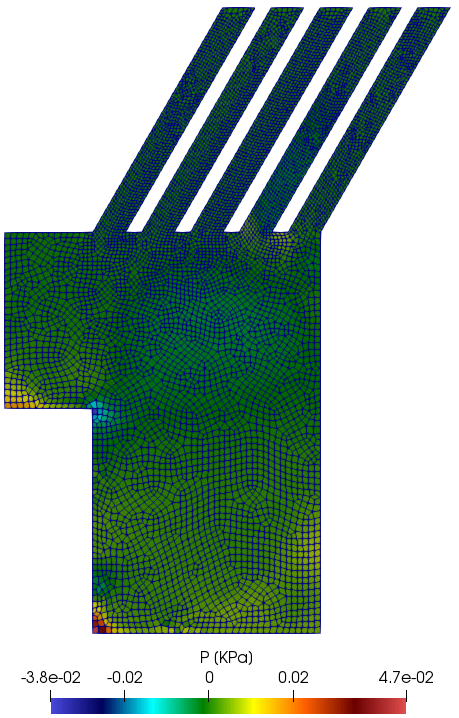
\includegraphics[width=0.42\textwidth]{Images/CFDEM/p.png}
	\caption{Diagrama de contorno de presi\'on $t=60 [s]$.}
	\label{CFDEM:p}
\end{figure}